\section{Computação Afetiva}

\citet{Pic98} definiu Computação Afetiva como uma ``computação relacionada,
surgida ou que influência as emoções''. Além disso, computadores com emoções
permitem aos mesmos um determinado nível de comportamento inteligente e
criatividade que seria impossível sem as emoções e esse é o principal desafio
dessa área. Logo, o seu entendimento pode explicar fenômenos como, por
exemplo, atenção, memória e outros.


Essa área é normalmente dividida em duas sub-áreas. A primeira estuda o
reconhecimento e a expressão de emoções dentro da Interação Homem-Computador;
a segunda, foca na síntese de emoções para aprimorar os seres robóticos e/ou
para estudar o comportamento humano por meio de simulações. Há muita
aplicabilidade dessas técnicas, por exemplo: a área que reconhece as emoções
pode ser utilizada para adaptar o sistema ao estado da pessoa permitindo ao
mesmo instruí-la, questioná-la, encorajá-la ou ocultar determinadas
informações consideradas irrelevantes.

O objetivo de \citet{bick2003relational} com o projeto \emph{Relational
Agents} é possibilitar aos usuários a criação de um relacionamento social e
emocional com longa duração.  Em \citet{bickmore2009virtual}, a confiança no
agente torna possível discutir tarefas mais importantes como melhoria da saúde
ou até a compra de uma casa. Outro trabalho na área de IHC é o reconhecimento
de emoções para aumentar a imersão em jogos, por exemplo permitindo ao próprio
jogo adaptar eventos ou trechos tornando-o mais divertido e realista.

\begin{figure}
  \begin{center}
    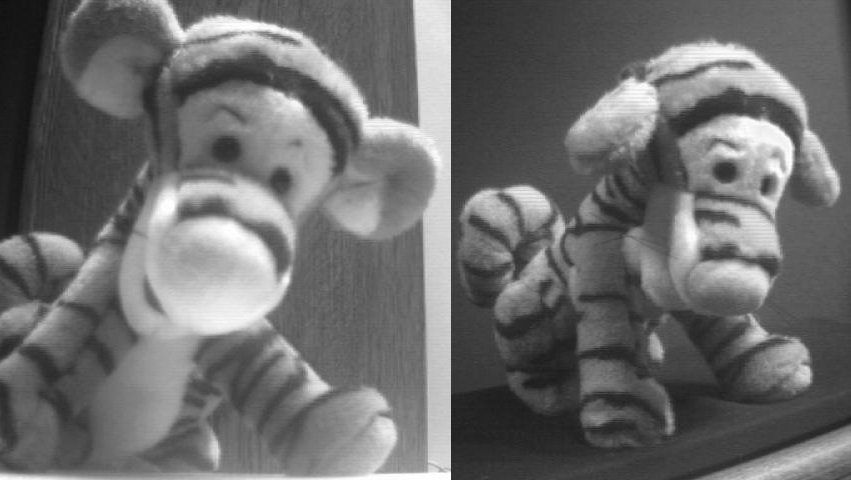
\includegraphics[width=75mm]{figuras/tigger-mit.png}
  \end{center}
  \caption{Brinquedo que responde as emoções das crianças \cite{kirsch1999affective}.}
  \label{fig:tigger-mit}
\end{figure}

O projeto \emph{The Affective Tigger: a reactive expressive toy} de
\citet{kirsch1999affective} é um brinquedo capaz de reconhecer e reagir às
emoções exibidas pelas crianças. Por exemplo, quando a criança encontra-se
feliz, o boneco expressa felicidade (ver Figura~\ref{fig:tigger-mit}). Ao todo
existem 5 estados emocionais: muito feliz, feliz, neutro, triste e muito
triste. Todos, com exceção do neutro, possuem alguma síntese vocal como um
rosnado (tristeza) ou uma risada (muito feliz). Assim, esse brinquedo, por ser
considerado um ser robótico que reage à criança com seus próprios estados
emocionais, fica enquadrado na segunda área.  Portanto, o desenvolvimento
desse brinquedo serviu para aprimorar os seres robóticos.

O projeto AIDA\footnote{Mais detalhes, ver http://senseable.mit.edu/aida} (do
inglês \emph{Affective Intelligent Driving Agent}) pode ser entendido como
enquadrado na área de IHC, pois o interesse é entender o estado afetivo da
pessoa dirigindo. Além disso, interessa-se em ter um relacionamento com o
usuário sugerindo alterações nas rotas baseado na rotina aprendida depois de
um mês de aprendizado.  A pesquisa relatada em \citet{dias-agents} visou
melhorar a simulação de agentes através do uso da emoção guiando o processo
deliberativo e melhorar o entendimento e gerência das emoções.  O presente
trabalho se enquadra na área de síntese de emoção, pois o interesse é em
entender o estado emocional e como ele pode afetar o comportamento de um
personagem.

\subsection{Modelo Cognitivo Emocional} % TI 2
\subsection{Ontologias Afetivas} % TI 2
\subsection{Arquiteturas Emocionais} % sao so as similares (usam o OCC)
\subsubsection{O Raciocinador Afetivo} % June 1992
% At least 2 pages
\subsubsection{Conjunto de Ferramentas Em} % May 1996 bates-based
% At least 2 pages
\subsubsection{Émile} % L? 2000
% At least 2 pages
\subsubsection{EMA} % P? 2004
% At least 2 pages
\subsubsection{ALMA} %K? 2005
% At least 2 pages
\subsubsection{FATIMA/fearNot!} % X? 2009/ Y? 2007
% At least 2 pages
\subsubsection{WASABI} % March? 2008
% At least 2 pages

